\documentclass{standalone}
\begin{document}
    
\subsection{Aufgabe 5.7}

a)\\
\noindent grün: $sin(4x)$, schwarz: $sin(3x)$, blau: $sin(2x)$, rot: $sin(x)$.\\

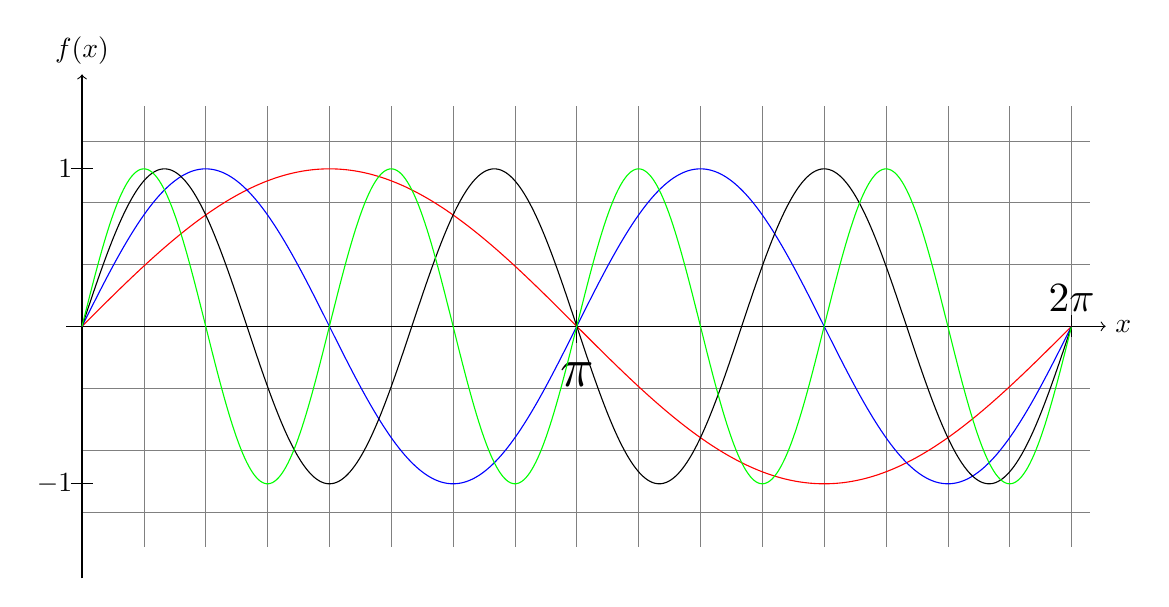
\begin{tikzpicture}[scale=2]
	
	\draw[very thin, gray, step=0.125*pi] (0, -1.4) grid (6.4, 1.4);
	
	\draw[->] (-0.1, 0) -- (6.5, 0) node[right] {$x$};
	\draw[->] (0, -1.6) -- (0, 1.6) node[above] {$f(x)$};
	
	\draw (1*pi, 3pt) -- (1*pi , -3pt) node [below, scale=2] {$\pi$};
	\draw (2*pi, 2pt) -- (2*pi , -2pt);
	\draw (2*pi, 0) node [above, scale=1.5] {2$\pi$};
	
	\draw (-2pt, 1) -- (2pt, 1);
	\draw (0, 1) node[left] {$1$};
	
	\draw (-2pt, -1) -- (2pt, -1);
	\draw (0, -1) node[left] {$-1$};
	
	\draw[domain=0:2*pi, red] plot[samples=500] (\x, {sin(\x r)});
	\draw[domain=0:2*pi, blue] plot[samples=500] (\x, {sin(2*\x r)});
	\draw[domain=0:2*pi] plot[samples=500] (\x, {sin(3*\x r)});
	\draw[domain=0:2*pi, green] plot[samples=500] (\x, {sin(4*\x r)});
	
\end{tikzpicture}\\

\newpage
\noindent b)\\
\begin{tabularx}{0.484\textwidth}
	{
		| >{\raggedleft\arraybackslash}c
		| >{\raggedleft\arraybackslash}c
		| >{\raggedleft\arraybackslash}c
		| >{\raggedleft\arraybackslash}c
		| >{\raggedleft\arraybackslash}c
		| >{\raggedleft\arraybackslash}c
		| >{\raggedleft\arraybackslash}c
		| >{\raggedleft\arraybackslash}c
		| >{\raggedleft\arraybackslash}c
		| >{\raggedleft\arraybackslash}c
		| >{\raggedleft\arraybackslash}c
		| >{\raggedleft\arraybackslash}c
		| >{\raggedleft\arraybackslash}c
		| >{\raggedleft\arraybackslash}c
		| >{\raggedleft\arraybackslash}c
		|}
	\hline
	&        &                        &                        &                        &                    &      \\
	$x$             & 0      & $\frac{\pi}{6}$        & $\frac{\pi}{4}$        & $\frac{\pi}{3}$        & $\frac{\pi}{2}$    & $\pi$\\ 
	&        &                        &                        &                        &                    &      \\
	\hline
	&        &                        &                        &                        &                    &      \\
	$f(x)=sin(x)$   & 0      & $\frac{1}{2}$          & $\frac{\sqrt{2}}{2}$   & $\frac{\sqrt{3}}{2}$   & 1                  & 0    \\ 
	&        &                        &                        &                        &                    &      \\
	\hline
	&        &                        &                        &                        &                    &      \\
	$g(x)=cos(x)$   & 1      & $\frac{\sqrt{3}}{2}$   & $\frac{\sqrt{2}}{2}$   & $\frac{1}{2}$          & 0                  & -1   \\  
	&        &                        &                        &                        &                    &      \\
	\hline
	&        &                        &                        &                        &                    &      \\
	$h(x)=tan(x)$   & 0      & $\frac{\sqrt{3}}{3}$   & 1                      & $\sqrt{3}$             & -                  & 0    \\ 
	&        &                        &                        &                        &                    &      \\
	\hline
	
\end{tabularx}

\end{document}